\setchapterpreamble[u]{%
    \margintoc\hfil
    \dictum[Richard Feynman]{What I cannot create,\\I do not understand.}
}

% Methods
\chapter{The spectrometer}
\labch{methods}
% Write in theorem-proof fashion

The individual parts of the spectrometer have been designed with several goals in mind. The main guiding principle was reproducibility and availability such that anyone can reproduce the build with minimal effort. All the necessary steps are documented below, including the reasoning for steps not taken. For verification and testing of the parts below the console (see \refsec{console}) itself may be used\sidenote{Instruction for using the RedPitaya as an \gls{lcrmeter}, \acrshort{vna}, or spectrum analyser can be found in its documentation}. A more practical solution is using separate devices for this to avoid the reconfiguration hassles. The open-source NanoVNA-H4\sidenote{\approx{}60CHF, \url{https://nanovna.com/}} \acrshort{vna} and the tinySA\sidenote{\approx{}50CHF, \url{https://tinysa.org/}} spectrum analyser are affordable and at these frequencies very capable alternatives to expensive lab equipment. They have been used extensively during the development of the hardware.

The following sections describe the design and build process --- including the reasoning behind the decisions taken --- of the \magnethical{} NMR spectrometer. \reffig{block-diagram} shows an overview schematic of the main components that will be discussed.

In general, the components were selected to be standard parts wherever possible. RF electronics are highly sensitive to stray capacitances and inductances, therefore most dedicated RF components use surface mount\sidenote{as opposed to through-hole (SMT)} (SMD) technology, sometimes even without pins. The passive components, like inductors, capacitors and resistors are in 0805\sidenote{0805 means \qty{0.08}{in} x \qty{0.05}{in}. PCB design is a mess of different unit systems, e.g. board sizes are often given in \unit{\milli\metre} whereas trace width is often given in \unit{mil} (thousandth of an \unit{in}). Rarely 0805 is written as 2012M: \qty{2.0}{\milli\metre} x \qty{1.2}{\milli\metre}} sizing, which was deemed large enough to be still easy to solder by hand. All traces were impedance matched to \qty{50}{\ohm} on standard \qty{1.6}{\milli\metre} FR4 cards, milled with standard drill sizes to facilitate the use of affordable standard manufacturing processes. Lastly, SMA connectors were chosen for their small footprint and secure screw connection, as opposed to BNC connectors (large) and SMB connectors (less secure connection). Most parts were searched for using the parametric search functionality of the big distributors and filtered for only active, available and stocked parts --- a rather large restriction in times of a global chip shortage.

\begin{figure}[hbt]
    \centering
    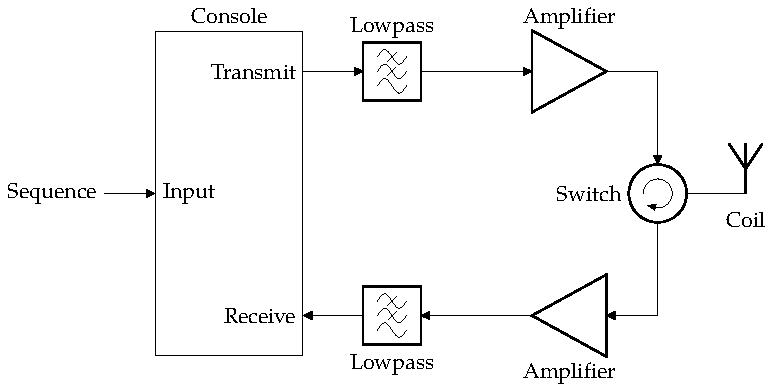
\includegraphics{images/block_diagram.pdf}
    \caption{\captiontitle{Block Diagram.} The main components of the \magnethical{} NMR spectrometer, including the console, lowpass filters, analogue amplifiers, transmit-receive switch and transmit-receive coil.}
    \labfig{block-diagram}
\end{figure}

The section order follows the path of the signal, that is, clockwise around the schematic starting with the console.

\section{The console}
\labsec{console}
\begin{marginfigure}[-4.5\baselineskip]
    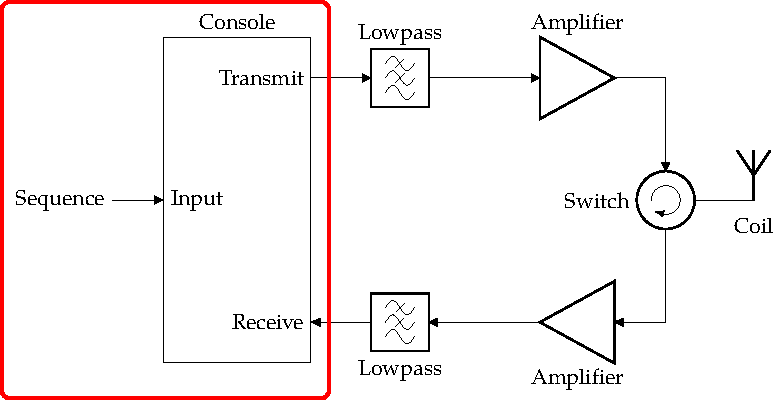
\includegraphics{block_diagram_highlight_console.pdf}
    \labfig{block-diagram-console}
\end{marginfigure}

The relatively low frequency of \(f_0 = \qty{25}{\mega\hertz}\)\sidenote{Given by the \ch{^1H} resonance frequency in the \qty{0.6}{\tesla} magnet} as well as the low bandwidth of only about \qty{10}{ppm}\sidenote{Equals \qty{25}{\hertz} at \qty{25}{\mega\hertz}} of the expected signal allows moving a lot of previously analogue tasks into the digital domain, greatly simplifying the hardware setup and making it more flexible. According to the Nyquist theorem, the minimum frequency that can be used to digitize an analogue signal without loss of information\sidenote{That is, without aliasing issues} must be more than twice as large as the highest frequency component of interest in the signal. In our case, the analogue-to-digital conversion must happen with more than
\[
    f_{min} \ge 2f_0 = \qty{50}{\mega\hertz}
\]
if oversampling is to be used. The setup could also make use of the low bandwidth of the signal and use the aliasing effect of the analogue-to-digital conversion to its advantage using undersampling. Since this requires taking further care when sampling and filtering, and the expected frequencies are low enough to make oversampling feasible, oversampling is employed in this setup. This has the added advantage of higher flexibility since the sampling frequency can be easily adjusted downwards.

For digital processing, a \acrfull{fpga} is used, which can be thought of as a piece of programmable hardware. To ease development a ready-made \acrshort{fpga} board --- the RedPitaya SDRlab 122-16 shown in \reffig{redpitaya} --- was chosen. With a sampling frequency of \qty{122.88}{\mega\sample\per\second} it is well above the Nyquist limit. Combined with a resolution of \qty{16}{bit} it is more than capable of capturing all relevant data from the analogue signal. Due to the commercial nature, the board is easily procured directly from RedPitaya or any of the well-known distributors\sidenote{For example Digikey, Mouser, Farnell, \dots}. A possible open-source alternative in the future would be the LimeSDR\sidenote{\url{https://limemicro.com/products/boards/limesdr/}}. With a sampling frequency of \qty{61.44}{\mega\sample\per\second}, limited by the USB3 interface, and a resolution of \qty{12}{bit} it is less powerful than the RedPitaya, but still fast enough for oversampling without loss of information. This board would cost less than half (\approx 280CHF) of the RedPitaya board and would enable a completely open design of the spectrometer --- in line with the accessibility goals of this work. Unfortunately, due to the young age of this project and the crowd-sourced nature, no board was available for purchase at the time of writing.

\begin{figure}[hbt]
    \centering
    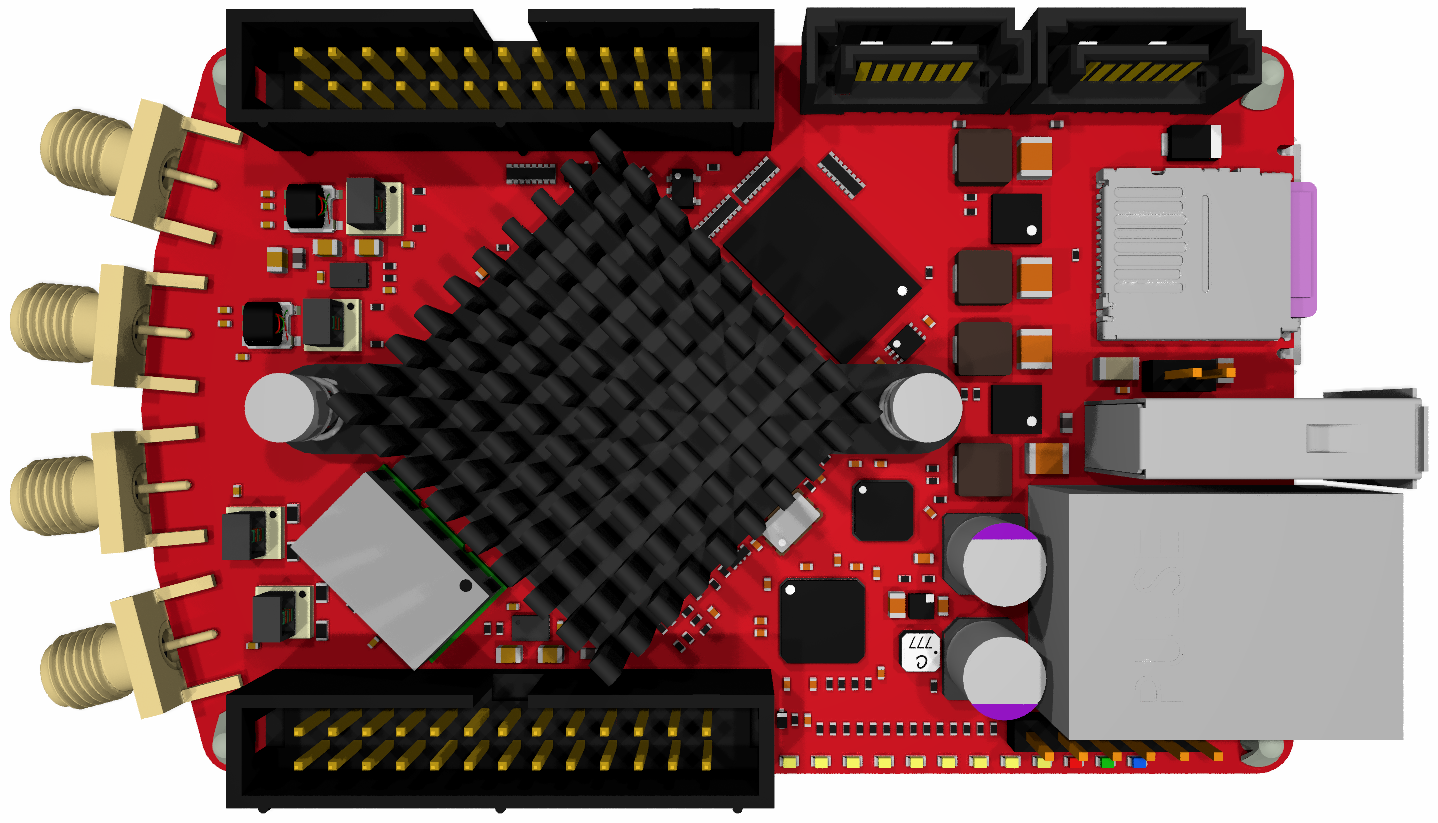
\includegraphics{images/rp122-16.png}
    \caption{\captiontitle{RedPiaya SDRlab 122-16.} 3D rendering of the console in KiCAD. Can be thought of as an \enquote{RF Raspberry Pi}. It has a Dual Core ARM Cortex A9, \qty{512}{\mega\byte} RAM, Gigabit Ethernet, 2x transmit, 2x receive, an ADC sample rate of \qty{122.88}{\mega\sample\per\second}, \qty{16}{\bit} resolution, a bandwidth of \qty{300}{\kilo\hertz} to \qty{550}{\mega\hertz} and a voltage range of \qty{0.5}{Vpp}/\qty{-2}{\deci\belm} (\qty{50}{\ohm}). The DAC has the same sample rate and voltage range, but a resolution of \qty{14}{\bit} and a bandwidth of \qty{300}{\kilo\hertz} to \qty{60}{\mega\hertz}.}
    \labfig{poweramp}
\end{figure}

After sampling the signal is demodulated using a quadrature detection system by multiplying it with the signal of a complex numerically controlled local oscillator. The same principle is applied inversely on the sending side for modulation. The resulting complex demodulated signal is then passed through a \acrfull{cic} filter for low-pass filtering and decimation to filter out high-frequency components of the signal and reduce the size of the data stream. The full data steam would incur a bandwidth of
\[
    \qty{16}{\bit} \cdot \qty{122.88}{\mega\sample\per\second} = \qty{245.76}{\mega\byte\per\second}
\]
per channel. With potentially 2 transmit and 2 receive channels this results in a data rate of close to \qty{1}{\giga\byte\per\second}, which is way higher than the theoretical limit of \qty{116}{\mega\byte\per\second} of the Ethernet interface. Due to inefficiencies in the Linux kernel of the RedPitaya Image, the practical data rate limit for continuous streaming is a lot lower at about \qty{20}{\mega\sample\per\second}\sidenote{According to the official \gls{lcrmeter} documentation (\url{https://redpitaya.readthedocs.io/en/latest/appsFeatures/applications/streaming/appStreaming.html})}. This has been improved in Pavel Demin's kernel image, where speeds up to \qty{80}{\mega\byte\per\second} have been measured\sidenote{\url{https://pavel-demin.github.io/red-pitaya-notes/alpine/}}. However, this only becomes relevant on long acquisition times over several seconds and hasn't been thoroughly tested as it hasn't been relevant, yet.

All of these digital signal-processing tasks are performed by the \acrshort{marcos} \acrshort{fpga} firmware developed by Vlad Negnevitsky\sidecite{negnevitskyMaRCoSOpensourceElectronic2023}. The system is designed for a low-field MRI system but could be easily adapted for NMR spectroscopy. The demodulated, filtered and decimated data from MaRCoS is then sent through its C server to the developed high-level Python interface. \reffig{marcos} shows an overview of the \acrshort{marcos} architecture. For more information on the Python programming interface see \refsec{software}.

\begin{figure}[hbt]
    \centering
    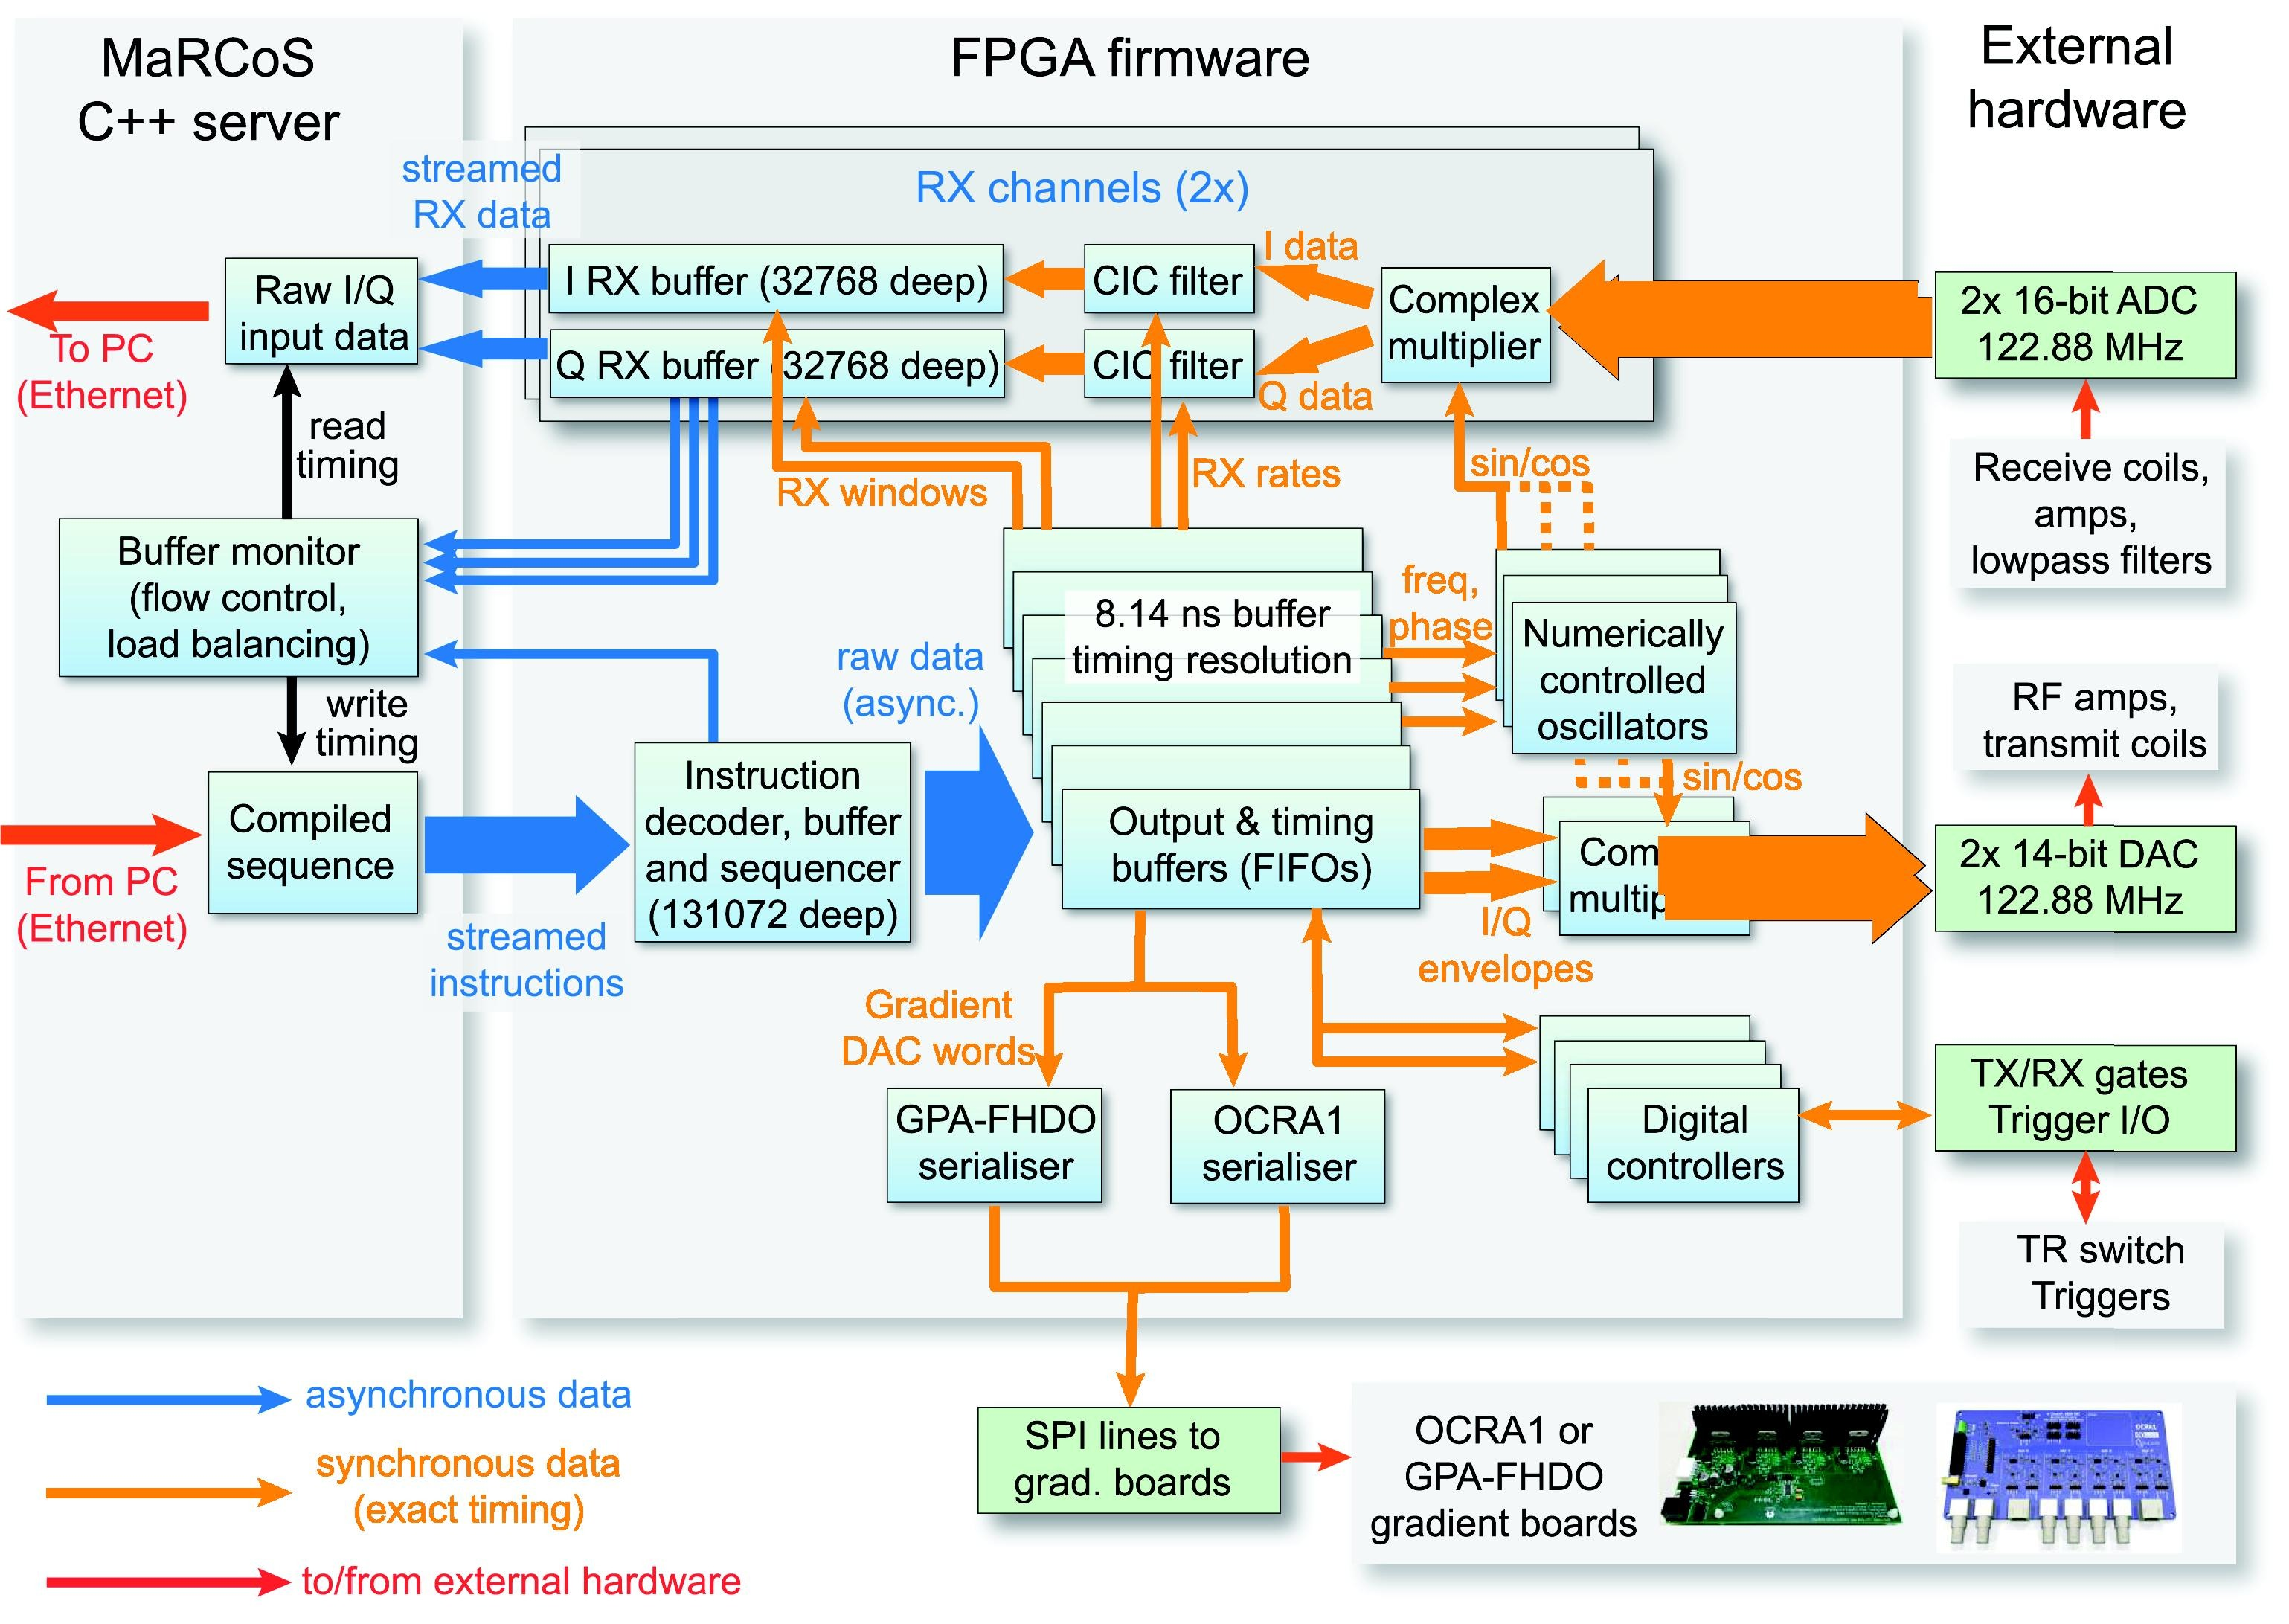
\includegraphics{images/marcos.jpg}
    \caption{\captiontitle{MaRCoS system architecture.} \enquote{The server receives a sequence from the client PC via Ethernet and streams it to the FPGA firmware, where it is translated into time-synchronous hardware operations including RF and gradient outputs. The firmware receives data from the ADCs, demodulates and filters it, and saves it into RX buffers, from which it is read by the server and sent to the PC} \cite{negnevitskyMaRCoSOpensourceElectronic2023}, Figure 3}
    \labfig{marcos}
\end{figure}

\section{The power amplifier}
\begin{marginfigure}[-4.5\baselineskip]
    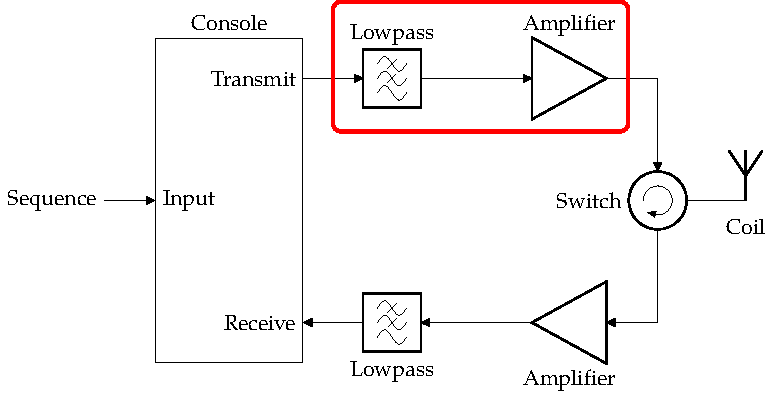
\includegraphics{block_diagram_highlight_tx.pdf}
    \labfig{block-diagram-pa}
\end{marginfigure}

The power amplifier has to amplify the low-power digitally synthesised signal from the console. The console described in \refsec{console} above has a maximum output power of \qty{0.5}{\volt} or \qty{-2}{\deci\belm} into a \qty{50}{\ohm} load.

The output power required to excite a volume of \qty{1}{\centi\meter\cubed} on a bandwidth of about \qty{10}{\kilo\hertz} or \qty{20}{ppm} in a high field magnet (\qty{500}{\mega\hertz} (\ch{^1H})/\qty{11.7}{\tesla}) is about \qty{11}{\watt} \sidecite{louis-josephDesigningBuildingLowcost2019}. The magnet in this work (see \refsec{magnet}) has a field strength of \qty{25}{\mega\hertz} (\ch{^1H})/\qty{0.6}{\tesla}, therefore \qty{20}{ppm} equals an excitation bandwidth of only \qty{500}{\hertz}. The sample Volume is only \(\qty{100}{\micro\litre} = \qty{0.1}{\centi\meter\cubed}\) as well, reducing the required energy further.

Targeting a pulse length of \qty{20}{\micro\second} for a \ch{^1H} \(\frac{\pi}{2}\)-pulse the RF pulse needs to generate a magnetic field of about
\[
    B = \frac{\alpha}{\gamma\tau} = \frac{\frac{\pi}{2}}{\qty{42.577}{\mega\hertz\per\tesla}\cdot{}\qty{20}{\micro\second}} = \qty{1.845}{\milli\tesla}
\]

The magnet has a homogenous region of \(\qty{100}{\micro\litre}\) for a \qty{5}{\milli\meter} NMR tube, resulting in an NMR active length of about \(l = \qty{6}{\milli\meter}\). If we assume a simple solenoid of that length with about \(n = 20\) turns, a Q factor of 100 (usually in the range of 10 to 1000 \sidecite{mispelterNMRProbeheadsBiophysical2015}) and a self-inductance of \(L = \frac{\mu_0n^2A}{l} = \qty{3}{\micro\henry}\)\sidenote{} we can roughly estimate the required peak power \(P\) with the following formulas \cite{mispelterNMRProbeheadsBiophysical2015}
\begin{align}
    B & = \frac{\mu{}_0nI}{l}              \\
    P & = R\underbar{I}^2 = R\frac{I^2}{2} \\
    Q & = \frac{L\omega}{R}                \\
\end{align}
where \(B\) is the magnet field produced by the current \(I\) through a solenoid of length \(l\) with \(n\) windings and and air core of permittivity \(\mu{}_0\). \(P\) is the maximum power pushed into the solenoid by current \(I\) over resistance \(R\) and \(Q\) is the definition of the quality factor for a self-inductance \(L\) and resistance \(R\). Putting it all together results in an estimated power level of
\begin{align}
    P & = \frac{B^2l^2L\omega}{2\mu{}_0^2n^2Q}                                                                                                                                              \\
      & = \frac{(\qty{1.845}{\milli\tesla})^2 \cdot (\qty{6}{\milli\metre})^2 \cdot \qty{3}{\micro\henry} \cdot 2\pi{} \cdot \qty{25}{\mega\hertz}}{2 \cdot \mu{}_0^2 \cdot 20^2 \cdot 100} \\
      & = \qty{457.12}{\milli\watt}
\end{align}

The exact power required is difficult to calculate at best due to various losses of the materials, the sample, the surrounding materials and losses due to radiation. Previous works with low-field NMR spectrometers used power amplifiers with a maximum power output of \qty{1}{\watt}\cite{chenUltralowCostNMR2015} and \qty{5}{W}\cite{louis-josephDesigningBuildingLowcost2019}. Lower power RF amplifiers have the advantage of lower required voltages, lower noise, less cooling requirements and simpler integrated designs.

The most affordable option for the power amplification would be based on \acrshort{rf} transistors. Unfortunately, this also necessitates an involved design process including not only biasing and feedback design, but also impedance matching and power supply circuits of a possible multi-stage power amplifier. This alone could be the topic of another thesis. Therefore, an \acrshort{mmic} approach has been chosen. Furthermore, availability in the \qty{1}{\watt} range is large due to a large commercial market in this power range especially for CATV amplifiers. Therefore, a \qty{1}{\watt} \acrshort{mmic} amplifier was chosen.

The \acrfull{mmic} amplifier has biasing, possible feedback and stabilization requirements all integrated on a single substrate design. In an application-only power, \acrshort{dc} blocking and adequate cooling have to be supplied since this is a Class A amplifier design.

The final board can be found in \reffig{poweramp}, with its schematic in the appendix \refsec{poweramp-schematic} and the part list in \refsec{poweramp-parts}.

\begin{figure}[hbt]
    \centering
    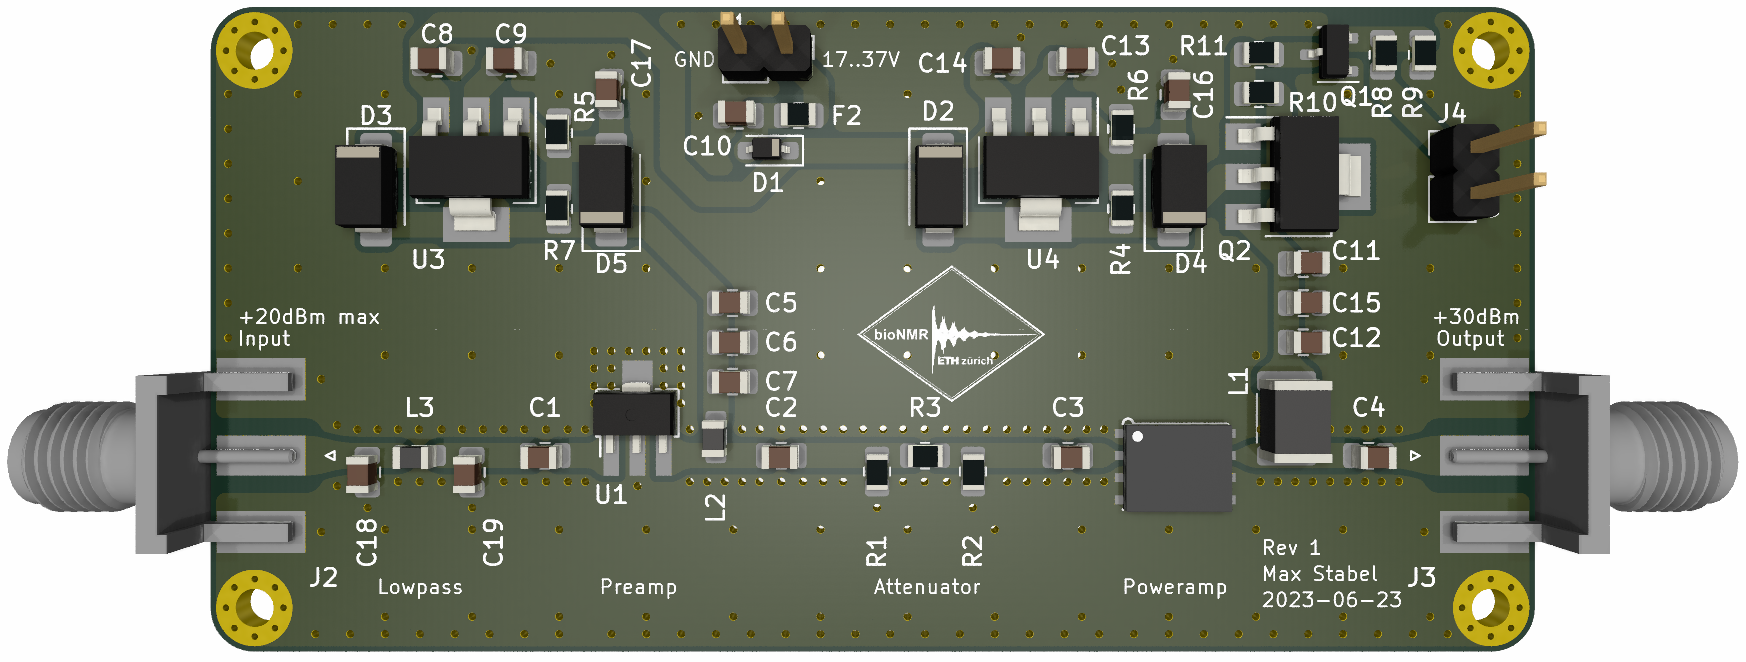
\includegraphics{images/poweramp.png}
    \caption{\captiontitle{\acrshort{rf} power amplifier.} 3D rendering of the power amplifier \acrshort{pcb} in KiCAD. The signal travels from left to right with the power supply circuitry above. It contains two \acrshort{mmic} amplifier stages, the AD5536 and the PHA-202+. A \qty{-6}{\deci\bel} attenuator was added in between and a passive low-pass filter in front (\(f_c = \qty{35}{\mega\hertz}\)). \(G \approx \qty{32}{\deci\bel}\), \(P_{\qty{1}{\deci\bel}} \approx \qty{+30}{\deci\belm}\)}
    \labfig{poweramp}
\end{figure}

The signal from the RedPitaya travels left to right through a low pass, the pre-amplifier, an attenuator and the power amplifier. The parts at the top of the board are standard linear voltage regulators used for stabilizing the voltage from the external DC supply. The power amplifier chip itself can be switched off by cutting the voltage supply.

The low-pass input filter functions as a digital reconstruction filter, smoothing the digitally synthesised waveform by filtering out high-frequency components of the signal left over from the switching of the FPGA and the zero-order hold DAC chip. It's a passive Chebyshev low-pass LC ladder filter realized with three 0805-sized SMD components.

The power amplifier is a PHA-202+, chosen for its easy powering requirements, \qty{50}{\ohm} matching and wide availability. However, it doesn't have enough gain (\qty{18.3}{\deci\bel})) to take the signal from \qty{-2}{\deci\belm} all the way to \qty{+30}{\deci\belm}. The missing \qty{14}{\deci\bel} in amplification are provided by the preamp (\qty{20}{\deci\bel}) minus the following attenuator (\qty{6}{\deci\bel}).

The AD5536 pre-amplifier is a \qty{50}{\ohm} matched, widely available \qty{20}{\deci\bel} gain GaAs gain block from Analog Devices. It's in an easy-to-solder package and has a low enough frequency specification to work with \qty{25}{\mega\hertz}. Alternatives with this gain and power are often difficult to solder due to the leadless design, unmatched (e.g. AFIC901N) \qty{75}{\ohm} matched (e.g. MAAL-011139) and often can't amplify such a slow signal (e.g. TAT7430B, starting at \qty{50}{\mega\hertz}).

The \qty{6}{\deci\bel} resistive attenuator in between the amplifiers is realized as a \(\pi\)-circuit similar to the low pass ladder filter. It is used to stabilize the adjacent amplifiers and will dampen any oscillations that might occur due to load or stray capacitances or inductances. If necessary the attenuation could be reduced to e.g. \qty{3}{\deci\bel} to increase the maximum power output of the amplifier, however, since the \(P_{\qty{1}{\deci\bel}} = \qty{29}{\deci\belm}\) for the PHA-202+ it won't grow linearly. The potential distortions should be of little consequence for the transmission signal.

For blocking the DC bias current for the amplifiers simple 0805 100nF caps are used in series as a high pass filter. For a \qty{50}{\ohm} system we can calculate the minimum value for the capacitors using the standard formula \(X_C = \frac{1}{2\pi{}fC}\) and keeping in mind that the block is loaded on both sides thus \( 2 \cdot \qty{50}{\ohm} = \qty{100}{\ohm}\). For \qty{25}{\mega\hertz} we thus get a minimum capacitance of
\[
    C = \frac{1}{2\pi{}fX} = \frac{1}{2\pi{} \cdot{} \qty{25}{\mega\hertz} \cdot{} \qty{100}{\ohm}} = \qty{63.7}{\pico\farad}
\]
The chosen \qty{100}{\nano\farad} are significantly larger and simply chosen for convenience and availability. Their high-pass cut-off frequency is at
\[
    f = \frac{1}{2\pi{}XC} = \frac{1}{2\pi{} \cdot{} \qty{100}{\ohm} \cdot{} \qty{100}{\nano\farad}} = \qty{15.9}{\kilo\hertz}
\]
For the chosen capacitors\sidenote{C0805C104J5RACTU} by KEMET this can be easily verified using the provided K-SIM simulator\sidenote{\url{https://ksim3.kemet.com/capacitor-simulation}}, which confirms an insertion loss (S21) of \qty{0}{\deci\bel} and an input reflection (S11) of \qty{-68}{\deci\bel} for \qty{25}{\mega\hertz}.

\section{The switch}
\begin{marginfigure}[-4.5\baselineskip]
    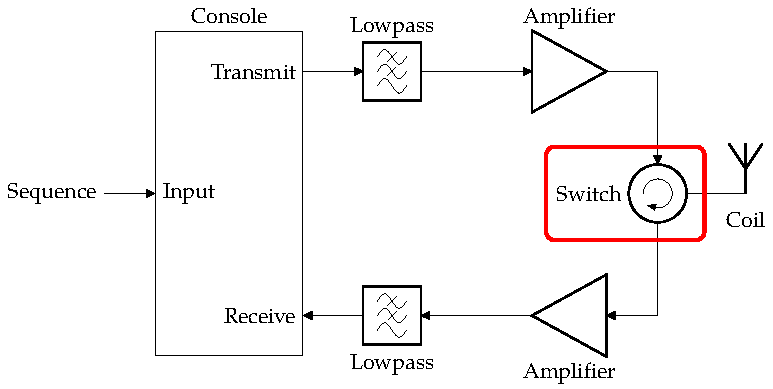
\includegraphics{block_diagram_highlight_switch.pdf}
    \labfig{block-diagram-switch}
\end{marginfigure}
building of the switch

\begin{figure}[hbt]
    \centering
    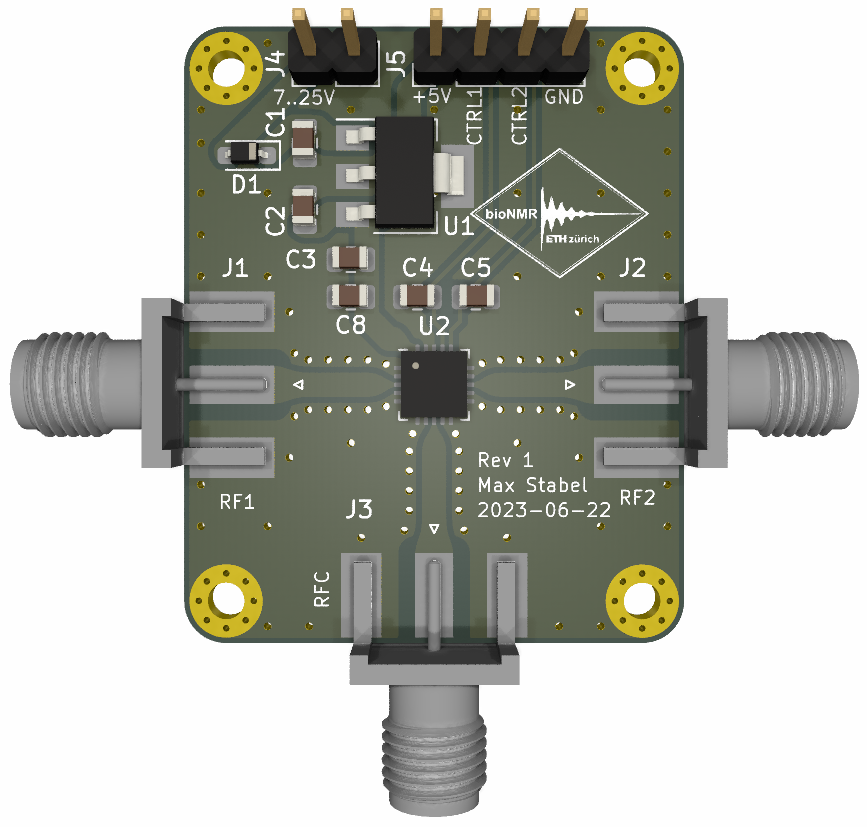
\includegraphics{images/tr_switch.png}
    \caption{\captiontitle{\acrshort{rf} \acrshort{tr} switch} 3D rendering of the switch \acrshort{pcb} in KiCAD. The transmit and receive amplifiers are connected on the left and right, the probe at the bottom connector. The central part is a Qorvo QPC6324 \acrfull{spdt} switch. Above it is a linear power supply and connection pins for active switching and power supply.}
    \labfig{switch}
\end{figure}


\section{The probe}
\begin{marginfigure}[-4.5\baselineskip]
    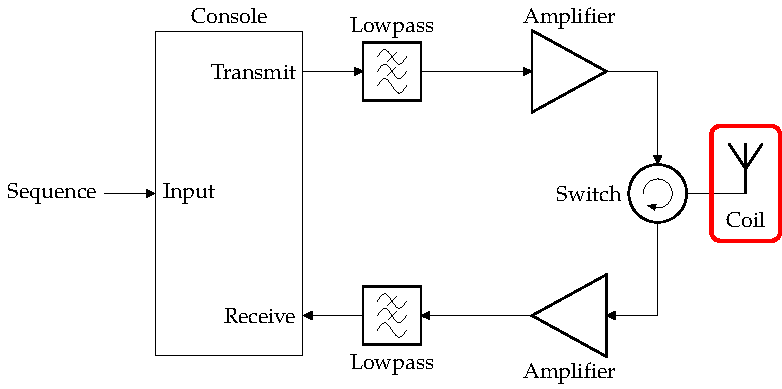
\includegraphics{block_diagram_highlight_coil.pdf}
    \labfig{block-diagram-coil}
\end{marginfigure}
building the coil

Solenoid is probably the best design in terms of sensitivity for NMR, but inductance increases rapidly with the dimensions. Thus it is best used for small samples and/or low fields\cite{mispelterNMRProbeheadsBiophysical2015}.

Assuming a long coil magnetic field is estimated by
B = u0 * n * I / l \cite{mispelterNMRProbeheadsBiophysical2015}

\begin{figure}[hbt]
    \centering
    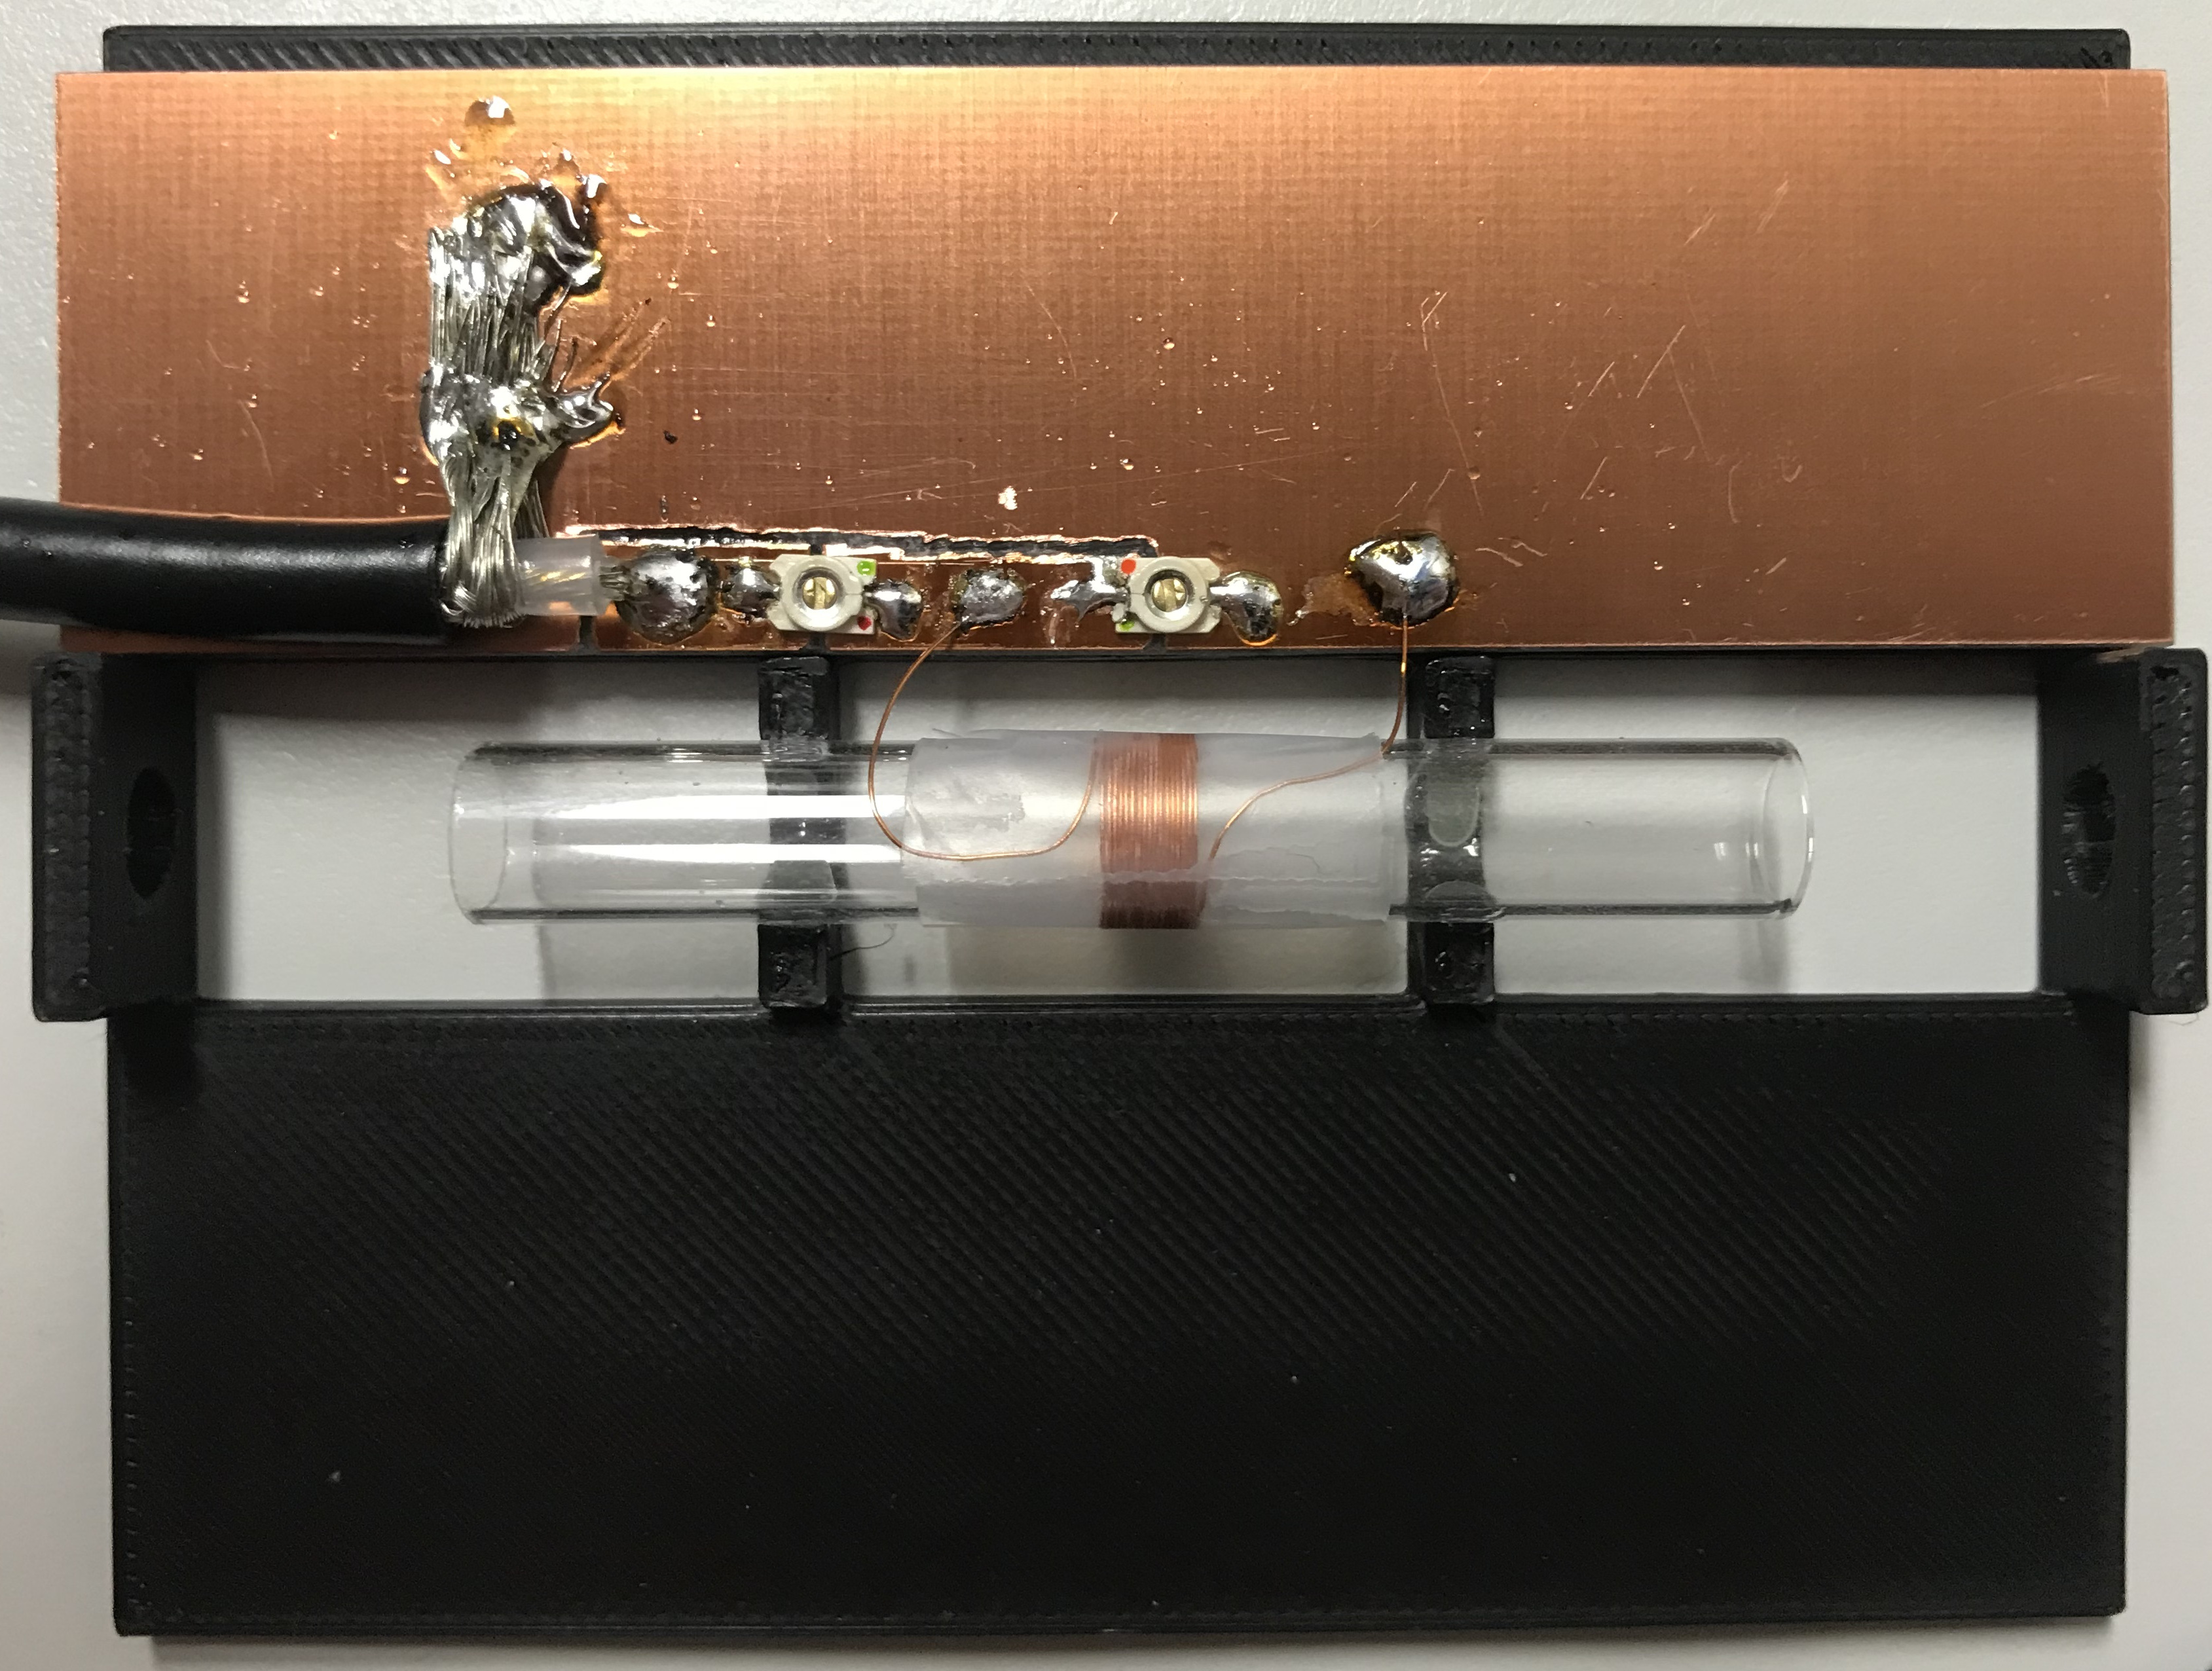
\includegraphics{images/probe.jpg}
    \caption{\captiontitle{Probe holder and \acrshort{rf} coil with tuning and matching capacitors} The capacitors are tunable from \qtyrange{4.5}{20}{\pico\farad} of make JZ200HV. The coil has a diameter of \(d = \qty{7.5}{\milli\meter}\), wire diameter \(D = \qty{0.2}{\milli\meter}\) and \(n = \qty{18}{turns}\) on a length of \(l = \qty{4}{\milli\meter}\). It has a measured inductance of \(L_{\qty{1}{\mega\hertz}} = \qty{2.7}{\micro\henry}\) and a resistance of \(R_{\qty{1}{\mega\hertz}} = \qty{0.63}{\ohm}\). The body was 3D printed and the circuit cut by hand.}
    \labfig{probe}
\end{figure}

\section{The low noise amplifier}

Basically the same as the power amplifier, just lower noise.

Mention input filter

Mention protection diodes

\section{The 32-channel current source}
building the power supply
\begin{figure}[hbt]
    \centering
    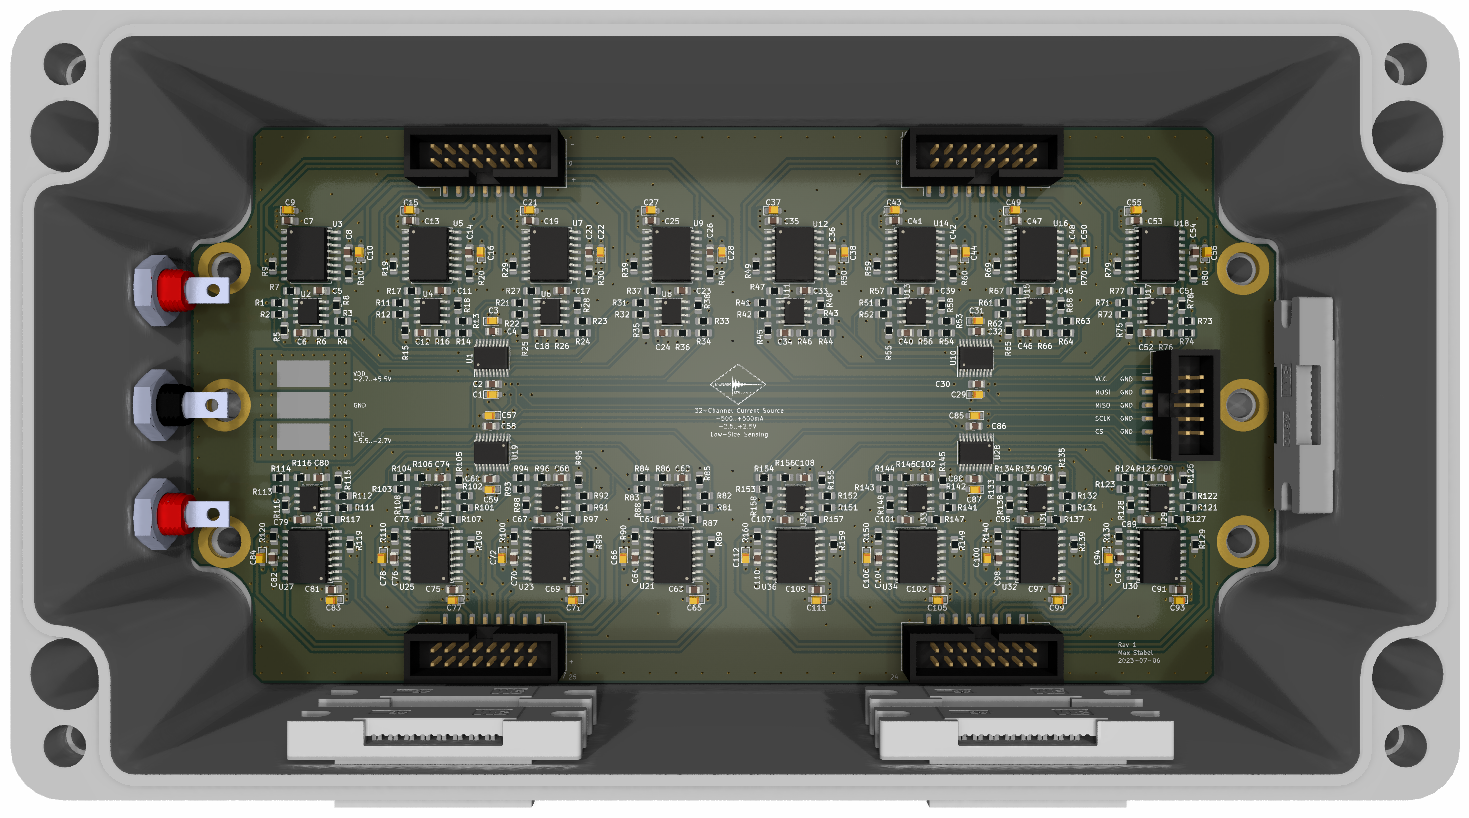
\includegraphics{images/32-channel_current_source.png}
    \caption{\captiontitle{32-channel programmable current source.} 3D rendering of the current source \acrshort{pcb} in \gls{kicad}. The \acrshort{spi} interface is on the right, the power connectors on the left and the 32 output channels on the top and bottom of the \acrshort{pcb}. It consists of 4 8-channel \acrshort{adc}s (AD5676R) setting a voltage that is converted to a constant current by two \acrshort{opamp}s: LMV358 for signal scaling and shifting and TCA0372 for the constant current source.}
    \labfig{current-source}
\end{figure}

\section{The magnet}
\labsec{magnet}
The magnet was built by SABR Enterprises, LLC with a homogenous volume of \qty{100}{\micro\litre} using a \qty{5}{\milli\metre} NMR tube. It has a field strength of \qty{0.6}{\tesla}/\qty{25}{\mega\hertz} with a homogeneity of at least \qty{0.1}{\partspermillion} inside the homogenous volume with the magnetic ink shims and active electronic shimming performed by NuevoMR, LLC\sidenote{spherical harmonic fields of order 1-4 (except \(XY(X^2-Y^2)\))}. A simple two-dipole setup is employed due to the ease of construction and shimming. The schematic can be found in the appendix \refsec{magnet-schematic}.

A Halbach array --- the so-called NMR Mandhala --- was considered as well. While the achievable field strengths of \qtyrange{0.5}{2}{\tesla} \sidecite{blumichCompactNMR2014} are sufficient, the initially achievable line width of \qty{700}{\partspermillion} \sidecite{raichDesignConstructionDipolar2004} (without shims) magnets is not\sidenote{The chosen dipole magnet achieved a homogeneity \qty{4.7}{\partspermillion} without active shims}. This can be compensated by further passive and active shimming, at the expense of adding complexity to the design. The shimming of Mandhala magnets is still ongoing research, e.g. \sidecite{danieliSmallMagnetsPortable2010}, \sidecite{parkerShimmingHalbachMagnets2016} or \sidecite{wangDesignShimmingMethod2022}. This design is worth investigating further in the future promising low sub-kg weighta as well as price reductions --- also considering the current price point for the dipole magnet of \approx \qty{9}{kCHF}.

For the material, temperature-compensated samarium cobalt (SmCo TC)\sidenote{EC 2:17-TC16} with a reversible temperature coefficient (RTC) of \qty{-0.001}{\%\per\kelvin} was chosen. The more common and cheaper Neodymium is more temperature sensitive with an RTC of around \qty{-0.1}{\%\per\kelvin}. Due to the low field, multiple scans will likely be required for at least some NMR measurements, exasperating the undesirable effect of a field drift over longer periods.

\section{The software}
\labsec{software}

Cite nmrglue here \sidecite{helmusNmrglueOpenSource2013}

design and development of the control software

short description of marcos? Already mentioned in console?


% Building process
% Lessons learned